\subsubsection*{QGIS}
Die Kartierungsvorgänge wurden alle mit der Free Open Source Software \emph{QGIS}\cite{qgis} durchgeführt.
\begin{figure}[ht]
    \centering
    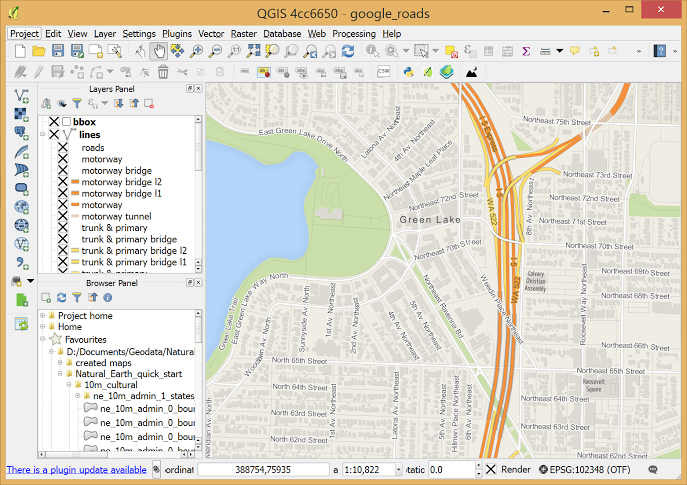
\includegraphics[width=6cm]{Images/QGIS/about-screenshot.png}
    \caption[fig:qgisabout]{QGIS-Benutzeroberfläche}
\end{figure}
\\Mithilfe dieser Software lassen sich basierend auf bereits existierenden Karten, 
wie beispielsweise OpenStreetMap\cite{ostrm} oder OpenSeaMap\cite{oseam}, eigene Routen sowie
Points of Interest(POIs) ohne großen Aufwand eintragen. Genauso leicht erfolgt der Import der von 
Navigationsgeräten der ALDEBARAN gespeicherten Routen. 
\subsubsection*{}
Die von der Schiffscrew und Prof. Dr. Greinert bereitgestellten Daten geben ein höchstakkurates Bild der
gefahrenen Route, inklusive der Schiffsposition und Geschwindigkeit (Speed Over Ground, ab hier SOG).
Somit können wir uns bei Sediment- und Wasserproben auf die Zeit, zu der diese genommen wurden, berufen,
ohne dass man die Koordinaten direkt mitschreiben müsste.
